% !TeX root = tlk16jun15h.tex
% !TeX encoding = UTF-8
% !TeX spellcheck = en_US


\input{../HEADER/HEADER}
% ********************************

\author{Alexander Maringele}
\title{flea\\
}
%\subtitle{of an instantiation-based first order theorem prover with equality}
\subtitle{bit(e)s and pieces}
%\subtitle{in easy examples}
\date{June 15th, 2016}
%======

%\includeonly{DiscriminationTree}
\begin{document}

\selectlanguage{english}

\input{../TitleFrame} 

\frame{
	
	
	\begin{quote}
		Hofstadter's Law: It always takes longer than you expect, 
		
		even when you take into account Hofstadter's Law.
	\end{quote}
	 \hfill--- Douglas Hofstadter, Gödel, Escher, Bach: An Eternal Golden Braid
	}

\frame{
	\setcounter{tocdepth}{1}
	\tableofcontents}

%\include{Title}
\section*{References}
\frame[<+->]{
\frametitle{References}

%\nocite{CS2011PhD}
\nocite{Dutertre:cav2014,BarFT-SMTLIB}
%\nocite{Hofstadter:1979:GEB:539932,NHRV2001ote}
%\nocite{ SRV2001ti,ZHM2009jar,RV2003eir,NHRV2001ote}	% ZHM2009jar, RV2003eir, NHRV2001ote
\bibliographystyle{amsalpha}
\bibliography{biblio}

}

% \cite{Hofstadter:1979:GEB:539932}

%\cite{GM2015ar}
%\cite{CS2011PhD}
%\cite{Lynch2013} % SMELS

%\cite{BarFT-SMTLIB}
%\cite{Dutertre:cav2014}
%\include{Overview}

%====================================================================
% BEGIN: CONTENT ----------------------------------------------------
%====================================================================

\section{Previously}

% !TeX root = tlk16jun15h.tex

\subsection{First-order refutation}

\begin{frame}
	% We transform a first formula in to a equisatisfiable set of clauses,
	% i.e. the conjunction of universally quantified disjunction of variable distinct first order literals
	% then we check if the set is satisfiable, if not then the formula is a theorem.
%	\frametitle{Goal}
	
	% !TeX spellcheck = en_US
% !TeX encoding = UTF-8

\begin{tikzpicture}[scale = 1, transform shape, draw=black, fill=black, thick, sloped]

	\draw[myarrow, ultra thick] (0,0) -- 
	node[pos=0, above] {$F$} 
	(2,0);
		
	% outer rectangle
	\draw[rounded corners=1.5mm,dotted] (0.5,3) rectangle (8.5,-3);
	% is F a theorem?
	\draw(1.9,2.7) node {Is $F$ a theorem?};
	
\pause
	% SLIDE Is S satisfiable?
	\node[colG] (S) at (1.1,-2.7) {\scriptsize$\lnot F \approx S$};
\pause
		\node (S) at (2.5,0) {$S$};
		

			% SLIDE 2
			\draw[thin,dashed,draw=colO] (2.5,0) ellipse (0.4 and 1.2); % S
			
			% inner rectangle
			\draw[very thick,draw=DarkGray]  (1.5,-2.25) rectangle (8,2.25); 
			% is S satisfaible?
			\draw (2.9,1.9) node {Is $S$ satisfiable?};
	
\pause
		% SLIDE unsatisfiable
		\draw[thin,dashed,draw=colO] (2.6,0) ellipse (0.6 and 1.44);  % S
		\draw[dashed, draw=colG, thick] decorate[decoration={snake}] {(1.4, 1) -- (8.2,0.6)};
		\draw[myarrow, draw=colHi, ultra thick] (6.5,1.8) -- 
			node[pos=0,below] {unsatisfiable}
			node[pos=0.85, above] {theorem} 
			(10,1.8) ;

\pause
		% SLIDE satisfiable
		\draw[thin,dashed,draw=colO] (2.8,0) ellipse (0.9 and 1.73);  % S
		\draw[dashed, draw=colG, thick]  decorate[decoration={snake}] { (1.4,-1)  --  (8.2,-0.6) };
		\draw[myarrow,draw=colLo, ultra thick] (7,-1.3) -- 
			node[pos=0, below] {satisfiable}
			node[pos=0.75, above] {not a theorem} (11,-1.3) ;
		 
\pause
		% SLIDE 5
		 \draw[thin,dashed,draw=colO] (3.2,0) ellipse (1.35 and 2.07); % S
		 	\draw[myarrow,draw=colNa, ultra thick] (7,0.15) -- 
		 	%	node[pos=0,above] {space out}
		 	node[pos=0,below] {time out}
		 	node[pos=0.85, above] {maybe} (10.5,0.15) ;

	\onslide<1->
\end{tikzpicture}
	
\end{frame}

\subsection{Resolution and InstGen}

\frame{
	\begin{Definition}[Ordered Resolution]
		% !TeX spellcheck = en_US
% !TeX encoding = UTF-8


\[
	\infer
	[]
	{(C \lor D)\sigma}
	{A \lor C& \lnot B\lor D}
%		\qquad
%		\infer[]
%		{C\sigma}
%		{A\lor\lnot B\lor C}
		\]
		where 
		\begin{center}
		$A\sigma$ strictly maximal in $\mcC\sigma$, $\lnot B\sigma$ maximal in $\mcD\sigma$, $\sigma=\mgu(A,B)$.
		\end{center}
		\end{Definition}
	
	\begin{Definition}[Inst-Gen]
	% !TeX spellcheck = en_US
% !TeX encoding = UTF-8


\[
	\infer
	[]
	{(L \lor C)\sigma\quad(\lnot L'\lor D)\sigma}
	{L \lor C& \lnot L'\lor D}
	\]
	where
	\[
		\sel(L\lor C) = L\qquad\sel(\lnot L'\lor D) = \lnot{L'}\qquad\sigma=\mgu(L,L')
	\]

\end{Definition}

%\begin{Example}[Unsatisfiable set of clauses]
%	$S = \{ \mP(x)\lor\lnot\mP(y), \lnot\mP(\ma),\mP(\mb)\}$
%\end{Example}
}

\subsection{Examples}
\frame{
	\begin{Example}[Resolution]
		\vspace{-1em}
		\[
\infer[x\mapsto \ma]{
	\infer[y\mapsto \mb]{\emptyclause}{
		\lnot\mP(y)&\mP(\mb)
		}
	}{\mP(x)\lor\lnot\mP(y)&\lnot\mP(\ma)
			}
			\]
		\end{Example}
		
			\begin{Example}[Inst-Gen]
				\vspace{-1em}
				\begin{align*}
	S_0\bot =&\  
	\{ 
	{\colHi\mP(\bot)} \lor \lnot\mP(\bot), 
	{\colHi\lnot \mP(\ma)}, 
	{\colHi\mP(\mb)} 
		\} \tag{satisfiable} \\
		&\quad 
		\infer[x\mapsto\ma]{
			\mP(\ma)\lor\lnot\mP(y)
			}{\mP(x)\lor\lnot\mP(y))&\lnot\mP(\ma)}
			\\
			S_1\bot \supsetneq&\  
			\{  
			{\colHi\lnot \mP(\ma)}, 
			{\colHi\mP(\mb)},
				{\colLo\mP(\ma)} \lor {\colHi \lnot \mP(\bot) } \}
				\tag{satisfiable}
				\\
				&\quad
				\infer[y\mapsto\mb]{
					\mP(\ma)\lor\mP(\mb)}{
					\mP(\mb)&\mP(\ma)\lor\lnot\mP(y)
					}
					\\
					S_2\bot \supsetneq&\ 
					\{ \lnot\mP(\ma), \mP(\mb), \mP(\ma) \lor \lnot\mP(\mb) \} \tag{unsatisfiable}
	\end{align*}
			\end{Example}
		}
		
	

		



\section{Procedure}

% !TeX root = tlk16jun15h.tex


\subsection{Run-Loop}

\frame{\begin{block}{Run-Loop}
%\begin{figure}[hbt]
\begin{center}
\begin{tikzpicture}[scale=0.75, transform shape]
\node[rectangle] (start) at (0,-4em) {};
\node (nc) [myrect] at (0,0) {new\\clauses};
\node (pc) [myrect] at (0,8em) {passive clauses};
\node (ab) [myrect] at (-8em,3.5em) {instantiation};
\node (gs) [myrect] at (-8em,8em) {SMT};
\node (un) [mycircle,colHi,very thick] at (-15em,8em) {un\-satis\-fiable};
\node (se) [myrect] at (-8em,12.5em) {selection};
\node (gc) [myrect] at (0em,16em) {given clause};
\node (ac) [myrect,dashed] at (-14em,16.5em) {active clauses};

\node (sl) [myrect, thick] at (8em,12.5em) {selected literal};
\node (us) [myrect,colO] at (8em,8em) {search for conflicts};
\node (sa) [mycircle, very thick,colLo] at (15em,8em) {satis\-fiable};
\node (su) [myrect] at (8em,3.5em) {substitution};

\node (parse) [myrect,dotted]  at (14em,-2em) {read\\file(s)};

\draw[myarrow, dotted] (parse) to [bend left=20] (nc);
\draw[myarrow] (nc) to (pc);
\draw[myarrow] (nc.west)  to [bend left=10] (ab);
\draw[myarrow] (ab) to (gs);
\draw[myarrow] (gs) to (un);
\draw[myarrow] (gs) to (se);
\draw[myarrow] (pc) to (gc);
\draw[myarrow] (se.north) to [bend left=10] (gc.west);
\draw[myarrow] (us) to (sa);
\draw[myarrow] (us) to (su);
\draw[myarrow] (su) to [bend left=10] (nc.east);
\draw[myarrow] (sl) to (us);
\draw[myarrow] (gc.east) to [bend left=10] (sl.north);
%\draw[myarrow,dashed] (gc.north) to [bend right=15](ac);
\draw[myarrow, dashed] (gc) to [bend right=20] (ac);

\path (nc) edge [myarrow,loop below, dashed] (nc)
 (parse) edge [myarrow, loop above, dotted] (parse)
 (19em,-2em) edge [myarrow,dotted](parse)
;
\end{tikzpicture}
%\caption{Inst-Gen loop with maximal completion}
%\label{fig:inst-gen-maxcomp}
\end{center}
%\end{figure}
\end{block}}

\subsection{Redundancy}
		\frame{
			\begin{block}{Subsumption}
				\vspace{-1em}
%				Subsumed clauses can be removed from a set of first order clauses without affecting satisfiability.
%				Proper instances of clauses affect the satisfiability of the set of ground instances.
				\begin{gather*}
					S = \{C, D, \ldots \}\qquad \exists\theta\ C\theta\subseteq D 
					\tag*{C subsumes D}\\
					 S \text{ satisfiable} 
					 \overset{\text{\colHi\cmark}}\iff (S \setminus D) \text{ satisfiable }
%					   \tag*{Resolution}
					   \\
					   \theta\text{ is proper, }
					S\bot \text{ satisfiable}\ 
%					{\colLo\overset{\text{\colLo\xmark}}{\colLo\Leftarrow \Rightarrow}}
					{\colLo\overset{\text{\xmark}}{\Leftarrow\Rightarrow}}\
					(S \setminus D)\bot \text{ satisfiable } 
%					\tag*{Inst-Gen}
					\\
					\theta\text{ is renaming, }
					S\bot \text{ satisfiable} 
					{\overset{\text{\colHi\cmark}}\iff}
					(S \setminus D)\bot \text{ satisfiable } 
					\end{gather*}
				\end{block}
			
			\begin{Example}[]
				\vspace{-1em}
					\begin{gather*}
\{ 	\mP(x,y), \lnot\mP(\ma,z) \} 
\qquad 
\{ 	\mP(x,y), \lnot\mP(\ma,z), {\colG\mP(\ma,z)} \} 
\\
	\{ \mP(\bot,\bot), \lnot\mP(\ma,\bot) \} 
	\qquad 
	\{ \mP(\bot,\bot), {\lnot\mP(\ma,\bot)},{\colLo\mP(\ma,\bot)} \}
					\end{gather*}
				
				\end{Example}
%							\begin{block}{}
%								Proper instances of clauses affect the satisfiability of the set of ground instances.
%							\end{block}
			}
			
			\subsection{Data structures}
			\frame{
				\begin{block}{data structures}
					\begin{enumerate}
						\item trees to represent clauses, literals and terms
						\item path indexing for fast retrieval of clashing selected literals
						\item discrimination trees for fast retrieval of clause variants
					\end{enumerate}
					
					\end{block}
				}
				
				\subsection{Path indexing}
				\frame{
					% !TeX root = tlk16jun15h.tex
% !TeX encoding = UTF-8
% !TeX spellcheck = en_US

\begin{gather*}
	\{
	\TI{1}\mP(\mf(x,x)),
	\TI{2}\mP(\mg(\ma,x)), 
	\TI{3}\mP(\mf(y,z)),
	\TI{4}\mP(\mg(\ma,y)), 
	\TI{5}\mP(\mf(y,x)), 
	\TI{6}\mP(\mg(y,a))
	\}
\end{gather*}
%
\begin{center}
	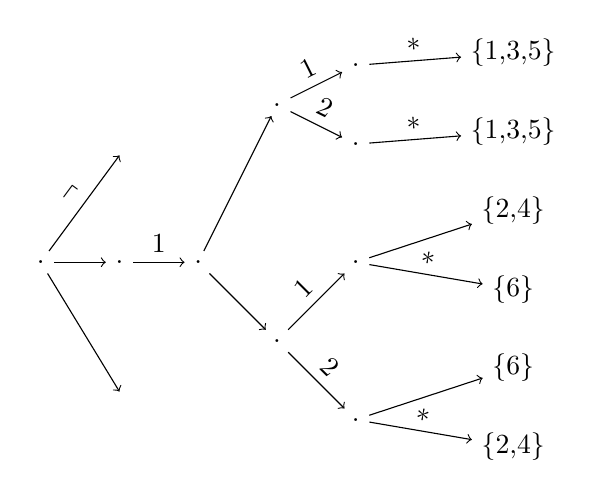
\begin{tikzpicture}[->,sloped,above]
	
	\node (root) at (0,2.5) {.};
	
	\node (h) at (1,2.5) {.};
	
	\node (h1) at (2,2.5) {.};
	
	\node (h1f) at (3,4.5) {.};
	\node (h1g) at (3,1.5) {.};
	
	\node (h1f1) at (4,5) {.};
	\node (h1f2) at (4,4) {.};
	\node (h1g1) at (4,2.5) {.};
	\node (h1g2) at (4,0.5) {.};
	
	\node (h1f1x) at (6,5) {\{1,3,5\}};
	\node (h1f2x) at (6,4) {\{1,3,5\}};
	\node (h1g1a) at (6,3) {\{2,4\}};
	\node (h1g1x) at (6,2) {\{6\}};
	\node (h1g2a) at (6,1) {\{6\}};
	\node (h1g2x) at (6,0) {\{2,4\}};
	
	\path (root) edge node {$\mP$} (h)
	(h) edge node {$1$} (h1)
	
	(h1)
	edge node {$\mf$} (h1f)
	edge node {$\mg$} (h1g)
	
	(h1f)
	edge node {$1$} (h1f1)
	edge node {$2$} (h1f2)
	
	(h1g)
	edge node {$1$} (h1g1)
	edge node {$2$} (h1g2)
	
	(h1f1)
	% edge node {$\ma$} (h1f1a)
	edge node {$*$} (h1f1x)
	
	(h1f2)
	%		edge node {$\ma$} (h1f2a)
	edge node {$*$} (h1f2x)
	
	
	(h1g1)
	edge node {$\ma$} (h1g1a)
	edge node {$*$} (h1g1x)
	
	(h1g2) 
	edge node {$\ma$} (h1g2a)
	edge node {$*$} (h1g2x)
	
	(root)
	edge node {$\lnot$} (1,4)
	edge node {$\mQ$} (1,1)
	;
	\end{tikzpicture}
\end{center}
$\lnot\mP(\mg(\mb,z)) \mapsto \{ \mP.1.\mg.1.{\mb}, \mP.1.\mg.2.{*} \} \mapsto \{6\} \cap \{2,4,6\}$}
				
				\subsection{Discrimination trees}
				\frame{
					% !TeX root = tlk16jun15h.tex
% !TeX encoding = UTF-8
% !TeX spellcheck = en_US

\begin{block}{}
	\def\TRIEWIDTH{4cm}
	\def\TEXTWIDTH{\textwidth-\TRIEWIDTH-2em}
	\begin{minipage}{\TEXTWIDTH}
		$
\TI{\ell_1}\mP(\mf(x,y)), 
\TI{\ell_2}\mP(\mf(x,\mh(\ma))),
\TI{\ell_3}\mP(\mf(\mh(\ma),\ma))
$
		\begin{align*}
			\ell_1 &\mapsto \mP.\mf.{*}.{*}\\
			\ell_2 &\mapsto \mP.\mf.{*}.\mh.\ma \\
			\ell_3 &\mapsto \mP.\mf.\mh.\ma.\ma
			\end{align*}
	\end{minipage}
	\begin{minipage}{\TRIEWIDTH}
		\def\pyL{-0.3}
		\def\pxL{-0.0}
		\begin{tikzpicture}[->,dotted]
		\renewcommand{\PAUSE}{}
		\input{DISCRIMINATIONTREE/Index}
		\node (lu) at (-3,-5.5) {} ;
		\end{tikzpicture}
	\end{minipage}
	%
\end{block}
					
					\begin{block}{Implementation}
						\vspace{-1em}
%						The literal index is implemented as mapping from yices literals to clauses.
						
						\begin{align*}
							\texttt{ Clause}&\mapsto\mathtt{(Int,\ Set\ of\ term\_t)}\\
						\texttt{ term\_t}&\mapsto \mathtt{Set\ of\ Int}\\
							\texttt{ Int}&\mapsto \mathtt{Clause}
						\end{align*}
						
						\end{block}
					}
					
\subsection{Yices API}
\begin{frame}
\scalebox{0.8}[1.0]{\begin{minipage}{40em}
\texttt{{\colEm type\_t} yices\_bool\_type({\colEm void});}
\\[0.25em]							
\texttt{{\colEm type\_t} yices\_new\_uninterpreted\_type({\colEm void});}
\\[0.25em]							
\texttt{{\colEm type\_t} yices\_function\_type({\colEm uint32\_t} n, const {\colEm type\_t} dom{\colEm []}, {\colEm type\_t} range);}
\\[0.75em]							
\texttt{{\colEm term\_t} yices\_new\_uninterpreted\_term({\colEm type\_t} tau);}
\\[0.25em]
\texttt{{\colEm term\_t} yices\_application({\colEm term\_t} fun, {\colEm uint32\_t} n, const {\colEm term\_t} arg[]);}
\\[0.25em]
\texttt{{\colEm term\_t} yices\_eq({\colEm term\_t} left, {\colEm term\_t} right);}
\\[0.75em]
\texttt{{\colEm term\_t} yices\_not({\colEm term\_t} arg);}
\\[0.25em]
\texttt{{\colEm term\_t} yices\_or({\colEm uint32\_t} n, {\colEm term\_t} arg{\colEm []});}
\\[0.75em]
\texttt{{\colEm int32\_t} yices\_assert\_formula({\colEm context\_t *ctx}, {\colEm term\_t} t);}
\\[0.75em]
\texttt{{\colEm smt\_status\_t} yices\_check\_context({\colEm context\_t *}ctx, const {\colEm param\_t *}params);}
\\[0.25em]
\texttt{{\colEm model\_t} *yices\_get\_model({\colEm context\_t *}ctx, {\colEm int32\_t} keep\_subst);}
\\[0.25em]
\texttt{{\colEm int32\_t} yices\_get\_bool\_value({\colEm model\_t *}mdl, {\colEm term\_t} t, {\colEm int32\_t *}val);}

\end{minipage}}
							
							
						
	
						\end{frame}

\section{Equality}
\frame{
	\begin{example}
		\vspace{-1em}
		\begin{align*}
%			
			S =&\ \{ \mP(\ma), \lnot\mP(\mf(\ma,\mb)), \mf(x,\mb)= x \} \\
%			
			&x=x \\
			{\colG x\neq y\ \lor}\ &y=x \\
			{\colG x\neq y \lor y\neq z\ \lor}\ &x=z
			\\
%			
			{\colG x_1\neq y_1 \lor x_2\neq y_2\ \lor}\ &\mf(x_1,x_2) = \mf(y_1,y_2) \\
		    {\colG x\neq y\ \lor}\ &\lnot\mP(x) \lor \mP(y)
			\end{align*}
		\end{example}
	
	}


\section{Bernays–Schönfinkel-Ramsey}

\subsection{Effectively Propositional}

\begin{frame}
	\begin{block}{}
		The Bernays–Schönfinkel-Ramsey class of first-order formulae is a decidable fragment of first-order logic.
%		 and can be effectively translated into propositional logic (EPR).
Each formulae in this fragment is equivalent to a formula
$\exists a_1\ldots a_m \forall y_1\ldots\ y_n F(a_1,\ldots,a_m,y_1,\ldots,y_n)$ 
where F is quantifier free and does not contain any function symbol,
which can easily transformed into
$\forall y_1\ldots\ y_n G(y_1,\ldots,y_n)$
where $G$ contains only constant function symbols.
		\end{block}
		
		
		
		\begin{example}
			\vspace{-1em}
			\begin{gather*}
				\ma\neq x\lor\mQ(\ma,x), \mQ(y,\mb)
			\end{gather*}
		\end{example}
	\end{frame}

\section{work to do}



\frame{
	\begin{itemize}
		\item migrate to Linux / Swift 3
		\item integrate unit superposition
		\item integrate ordered maximal completion 
		\item experiments
		\item optimizations
	\end{itemize}
	}
\subsection{optimization}

\frame{
	\begin{center}
	\includegraphics[scale=0.5]{../xkcd/optimization}
	\end{center}
	}
 
\end{document}